\begin{figure}[!htbp]
    \centering
    \begin{subfigure}[b]{0.25\textwidth}
        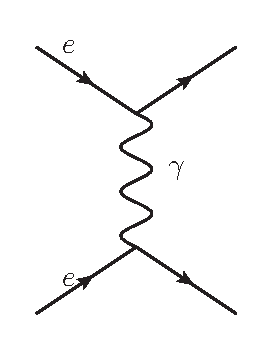
\includegraphics[width=\linewidth,scale=0.5]{figures/scattering.eps}
        \caption{}
        \label{fig:PhotonScattering}
    \end{subfigure}%
    \begin{subfigure}[b]{0.5\textwidth}
        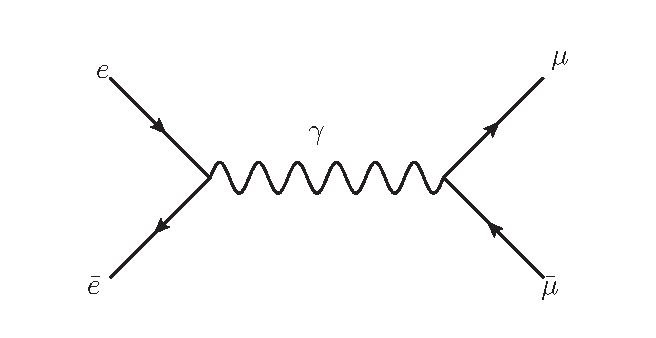
\includegraphics[width=\linewidth]{figures/fermionGammaTrans.eps}
        \caption{}
        \label{fig:FermionPhotonFussion}
    \end{subfigure}% 
    \begin{subfigure}[b]{0.3\textwidth}
        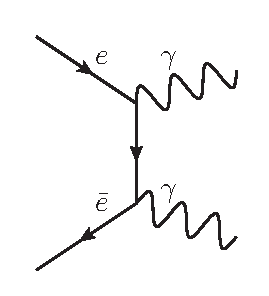
\includegraphics[width=\linewidth]{figures/annailation.eps}
        \caption{}
        \label{fig:PairAnnialation}
    \end{subfigure}%

    \caption[
        Photon interaction examples
    ]{
    Examples of interactions involving the photon. The left figure shows scatter, with two electrons repelling each other. The center demonstrates fusion, with electron/antielectron forming into a photon, which in turn becomes a muon/antimuon pair. The right figure is annihilation, where a electron/antielectron change into a pair of photons.
    }
    \label{fig:PhotonExamples}
\end{figure}